\section{Additional analyses}
\label{app:extra}

\paragraph{Models.} Table~\ref{tab:models} lists the model architectures. All models use grouped or multi-head attention; we average attention over query heads.
\begin{table}[H]\centering\small\caption{\textbf{Models.}}\label{tab:models}
\resizebox{\linewidth}{!}{\begin{tabular}{lrrrrr}
\toprule
Model & params & layers & heads & KV heads & hidden \\
\midrule
\texttt{Qwen/Qwen2.5-3B-Instruct} & 3.09B & 36 & 16 & 2 & 2048 \\
\texttt{Qwen/Qwen2.5-1.5B-Instruct} & 1.54B & 28 & 12 & 2 & 1536 \\
\texttt{microsoft/Phi-3-mini-4k-instruct} & 3.82B & 32 & 32 & 32 & 3072 \\
\texttt{TinyLlama/TinyLlama-1.1B-Chat-v1.0} & 1.10B & 22 & 32 & 4 & 2048 \\
\texttt{HuggingFaceTB/SmolLM-1.7B-Instruct} & 1.71B & 24 & 32 & 32 & 2048 \\
\texttt{mistralai/Mistral-7B-Instruct-v0.2} & 7.24B & 32 & 32 & 8 & 4096 \\
\texttt{Qwen/Qwen2.5-7B-Instruct} & 7.62B & 28 & 28 & 4 & 3584 \\
\bottomrule
\end{tabular}}
\end{table}

\paragraph{Length scaling of $1$D persistence on real attention.} Table~\ref{tab:scaling} regresses log total $1$D persistence (summed over layers) on $\log N$ with a class fixed effect, on rows with $P_1>0$, so that the exponent is not driven by a length difference between correct and hallucinated answers. Exponents range from 0.03 to 1.39, against 1.31 for i.i.d.\ uniform weights and 1.27 for random causal attention without a sink over the same range of $N$. 12 of the 13 fitted settings grow significantly more slowly than the i.i.d.\ reference (not HE Qw3B). The exponent exceeds $1$ in HE Qw1.5B and HE Qw3B, so growth on real attention is not uniformly sub-linear. TQA Mis7B and TQA Mis7B (chat) have too few rows with $P_1>0$ to fit (first column): almost all of their graphs are coned (Table~\ref{tab:theory}), so $1$D persistence is zero for almost every example whatever its length. In the other settings almost every example has some $1$D bar summed over layers, because those models have some layers that are not coned; within an example, the coned layers contribute nothing to $P_1$ whatever the length (Table~\ref{tab:theory}).
\begin{table}[H]\centering\small\caption{\textbf{Length scaling of $1$D persistence.} OLS of $\log P_1$ on $\log N$ and the class label, fit on the rows with $P_1>0$; the first column is the share of rows that are retained, and the rows with $P_1=0$ are dropped from the fit. Rows need per-example layer features, which we retain for 15 of the 16 settings (not TrQA Mis7B).}\label{tab:scaling}
\resizebox{\linewidth}{!}{\begin{tabular}{lrrrrr}
\toprule
Setting & rows with $P_1{>}0$ & $\hat\alpha$ (class FE) & 95\% CI & $R^2$ & Spearman$(P_1,N)$ \\
\midrule
TQA Qw3B & 100.0\% & 0.25 & [0.23, 0.27] & 0.27 & 0.57 \\
TQA Qw1.5B & 100.0\% & 0.57 & [0.52, 0.61] & 0.29 & 0.51 \\
TQA Phi-3 & 99.9\% & 0.93 & [0.82, 1.04] & 0.15 & 0.39 \\
TQA TinyLl. & 100.0\% & 0.32 & [0.28, 0.36] & 0.14 & 0.28 \\
TQA SmolLM & 100.0\% & 0.61 & [0.54, 0.69] & 0.13 & 0.36 \\
TQA Mis7B & 0.2\% & -- & -- & -- & -- \\
TQA Mis7B (chat) & 0.2\% & -- & -- & -- & -- \\
TQA Qw7B & 100.0\% & 0.59 & [0.55, 0.62] & 0.41 & 0.63 \\
HE Qw3B & 100.0\% & 1.39 & [1.31, 1.47] & 0.36 & 0.60 \\
HE Qw1.5B & 100.0\% & 1.10 & [1.07, 1.13] & 0.84 & 0.91 \\
TrQA Qw3B & 100.0\% & 0.72 & [0.68, 0.75] & 0.46 & 0.68 \\
TrQA Qw1.5B & 100.0\% & 0.75 & [0.72, 0.78] & 0.59 & 0.68 \\
TrQA Phi-3 & 100.0\% & 0.70 & [0.65, 0.75] & 0.29 & 0.49 \\
TrQA TinyLl. & 100.0\% & 0.03 & [0.02, 0.03] & 0.03 & 0.15 \\
TrQA Qw7B & 100.0\% & 0.84 & [0.81, 0.87] & 0.57 & 0.65 \\
\midrule
i.i.d.\ uniform weights (simulation) & 100\% & 1.31 & -- & -- & -- \\
random causal attention, no sink (simulation) & 100\% & 1.27 & -- & -- & -- \\
\bottomrule
\end{tabular}}
\end{table}

\paragraph{Sequence lengths.} Table~\ref{tab:lengths} gives class-conditional lengths. TruthfulQA is length-balanced by construction; HaluEval's hallucinated answers are systematically longer; on-policy, incorrect answers differ in length from correct ones because they are the model's own.
\begin{table}[H]\centering\small\caption{\textbf{Class-conditional sequence length} (mean $\pm$ SD, full sequence) and mean answer length. Rows need per-example layer features, which we retain for 15 of the 16 settings (not TrQA Mis7B).}\label{tab:lengths}
\resizebox{\linewidth}{!}{\begin{tabular}{lrrrrr}
\toprule
Setting & length $N$ (correct) & length $N$ (hallucinated) & answer tokens (c./h.) & point-biserial $r$ & Welch $p$ \\
\midrule
TQA Qw3B & $44.4\pm7.9$ & $44.0\pm8.0$ & 12.6 / 12.1 & -0.030 & 0.22 \\
TQA Qw1.5B & $44.4\pm7.9$ & $44.0\pm8.0$ & 12.6 / 12.1 & -0.030 & 0.22 \\
TQA Phi-3 & $29.2\pm8.9$ & $28.7\pm8.8$ & 11.8 / 11.4 & -0.024 & 0.32 \\
TQA TinyLl. & $42.5\pm9.0$ & $42.1\pm8.9$ & 12.1 / 11.7 & -0.024 & 0.32 \\
TQA SmolLM & $32.6\pm8.2$ & $32.1\pm8.2$ & 10.6 / 10.2 & -0.026 & 0.29 \\
TQA Mis7B & $33.3\pm8.7$ & $32.8\pm8.6$ & 11.4 / 10.9 & -0.029 & 0.25 \\
TQA Mis7B (chat) & $34.3\pm8.7$ & $33.8\pm8.6$ & 12.4 / 11.9 & -0.029 & 0.25 \\
TQA Qw7B & $44.4\pm7.9$ & $44.0\pm8.0$ & 12.6 / 12.1 & -0.030 & 0.22 \\
HE Qw3B & $121.2\pm39.7$ & $132.7\pm41.2$ & 3.8 / 15.4 & +0.141 & $2.1\times 10^{-10}$ \\
HE Qw1.5B & $122.2\pm39.5$ & $133.9\pm41.3$ & 3.6 / 15.3 & +0.144 & $5.1\times 10^{-6}$ \\
TrQA Qw3B & $68.0\pm10.4$ & $69.0\pm9.7$ & 5.3 / 5.7 & +0.052 & 0.02 \\
TrQA Qw1.5B & $67.5\pm10.3$ & $69.4\pm10.0$ & 5.4 / 5.9 & +0.086 & $1.3\times 10^{-4}$ \\
TrQA Phi-3 & $45.6\pm11.3$ & $46.9\pm11.2$ & 5.6 / 6.5 & +0.057 & 0.01 \\
TrQA TinyLl. & $67.3\pm12.5$ & $73.7\pm14.9$ & 17.0 / 19.6 & +0.196 & $1.8\times 10^{-21}$ \\
TrQA Qw7B & $67.4\pm9.6$ & $69.2\pm10.2$ & 5.0 / 5.5 & +0.092 & $3.8\times 10^{-5}$ \\
\bottomrule
\end{tabular}}
\end{table}

\paragraph{Margin sensitivity.} Table~\ref{tab:tost} reports TOST $p$-values at four equivalence margins for the four comparisons of Figure~\ref{fig:forest}; bold marks $p<0.05$ (equivalence).
\begin{table}[H]\centering\scriptsize\setlength{\tabcolsep}{2.2pt}\caption{\textbf{TOST $p$-values by margin $m$.} NT: all non-topological features.}\label{tab:tost}
\resizebox{\linewidth}{!}{\begin{tabular}{lcccccccccccccccc}
\toprule
Setting & \multicolumn{4}{c}{Sink vs.\ 0D} & \multicolumn{4}{c}{0D $\mid$ Sink} & \multicolumn{4}{c}{1D $\mid$ 0D} & \multicolumn{4}{c}{0D $\mid$ NT} \\
$m$ & {\scriptsize .010} & {\scriptsize .015} & {\scriptsize .020} & {\scriptsize .025} & {\scriptsize .010} & {\scriptsize .015} & {\scriptsize .020} & {\scriptsize .025} & {\scriptsize .010} & {\scriptsize .015} & {\scriptsize .020} & {\scriptsize .025} & {\scriptsize .010} & {\scriptsize .015} & {\scriptsize .020} & {\scriptsize .025} \\
\midrule
TQA Qw3B & \textbf{.029} & \textbf{.001} & \textbf{<.001} & \textbf{<.001} & \textbf{.040} & \textbf{.001} & \textbf{<.001} & \textbf{<.001} & 1.000 & .995 & .972 & .882 & \textbf{<.001} & \textbf{<.001} & \textbf{<.001} & \textbf{<.001} \\
TQA Qw1.5B & .109 & \textbf{.016} & \textbf{<.001} & \textbf{<.001} & .692 & .276 & \textbf{.040} & \textbf{.002} & .311 & \textbf{.034} & \textbf{<.001} & \textbf{<.001} & \textbf{<.001} & \textbf{<.001} & \textbf{<.001} & \textbf{<.001} \\
TQA Phi-3 & .138 & \textbf{.013} & \textbf{<.001} & \textbf{<.001} & .112 & \textbf{.003} & \textbf{<.001} & \textbf{<.001} & \textbf{<.001} & \textbf{<.001} & \textbf{<.001} & \textbf{<.001} & \textbf{<.001} & \textbf{<.001} & \textbf{<.001} & \textbf{<.001} \\
TQA TinyLl. & .520 & .234 & .064 & \textbf{.012} & .962 & .809 & .483 & .169 & .210 & \textbf{.021} & \textbf{<.001} & \textbf{<.001} & \textbf{<.001} & \textbf{<.001} & \textbf{<.001} & \textbf{<.001} \\
TQA SmolLM & .939 & .865 & .748 & .602 & 1.000 & .996 & .960 & .805 & .179 & \textbf{.036} & \textbf{.003} & \textbf{<.001} & \textbf{<.001} & \textbf{<.001} & \textbf{<.001} & \textbf{<.001} \\
TQA Mis7B & \textbf{<.001} & \textbf{<.001} & \textbf{<.001} & \textbf{<.001} & \textbf{<.001} & \textbf{<.001} & \textbf{<.001} & \textbf{<.001} & \textbf{<.001} & \textbf{<.001} & \textbf{<.001} & \textbf{<.001} & \textbf{<.001} & \textbf{<.001} & \textbf{<.001} & \textbf{<.001} \\
TQA Mis7B (chat) & \textbf{<.001} & \textbf{<.001} & \textbf{<.001} & \textbf{<.001} & \textbf{<.001} & \textbf{<.001} & \textbf{<.001} & \textbf{<.001} & \textbf{<.001} & \textbf{<.001} & \textbf{<.001} & \textbf{<.001} & \textbf{<.001} & \textbf{<.001} & \textbf{<.001} & \textbf{<.001} \\
TQA Qw7B & 1.000 & 1.000 & 1.000 & 1.000 & 1.000 & .999 & .964 & .719 & .962 & .836 & .578 & .281 & \textbf{<.001} & \textbf{<.001} & \textbf{<.001} & \textbf{<.001} \\
HE Qw3B & .910 & .676 & .351 & .110 & 1.000 & 1.000 & .982 & .804 & .906 & .551 & .148 & \textbf{.012} & \textbf{<.001} & \textbf{<.001} & \textbf{<.001} & \textbf{<.001} \\
HE Qw1.5B & .993 & .970 & .896 & .755 & .679 & .263 & \textbf{.041} & \textbf{.002} & .980 & .918 & .786 & .569 & \textbf{<.001} & \textbf{<.001} & \textbf{<.001} & \textbf{<.001} \\
TrQA Qw3B & .792 & .522 & .239 & .069 & .982 & .866 & .561 & .219 & .106 & \textbf{.015} & \textbf{.002} & \textbf{<.001} & \textbf{<.001} & \textbf{<.001} & \textbf{<.001} & \textbf{<.001} \\
TrQA Qw1.5B & .431 & .176 & \textbf{.050} & \textbf{.010} & .528 & .211 & \textbf{.044} & \textbf{.005} & .079 & \textbf{.011} & \textbf{<.001} & \textbf{<.001} & \textbf{<.001} & \textbf{<.001} & \textbf{<.001} & \textbf{<.001} \\
TrQA Phi-3 & \textbf{.047} & \textbf{.002} & \textbf{<.001} & \textbf{<.001} & .114 & \textbf{.005} & \textbf{<.001} & \textbf{<.001} & .086 & \textbf{.003} & \textbf{<.001} & \textbf{<.001} & \textbf{<.001} & \textbf{<.001} & \textbf{<.001} & \textbf{<.001} \\
TrQA TinyLl. & .091 & \textbf{.021} & \textbf{.003} & \textbf{<.001} & .071 & \textbf{.005} & \textbf{<.001} & \textbf{<.001} & .083 & \textbf{.013} & \textbf{.002} & \textbf{<.001} & \textbf{<.001} & \textbf{<.001} & \textbf{<.001} & \textbf{<.001} \\
TrQA Mis7B & .111 & \textbf{.023} & \textbf{.003} & \textbf{<.001} & .052 & \textbf{.004} & \textbf{<.001} & \textbf{<.001} & .315 & .096 & \textbf{.017} & \textbf{.002} & \textbf{<.001} & \textbf{<.001} & \textbf{<.001} & \textbf{<.001} \\
TrQA Qw7B & .993 & .982 & .962 & .924 & .959 & .852 & .606 & .314 & .054 & \textbf{.007} & \textbf{<.001} & \textbf{<.001} & \textbf{<.001} & \textbf{<.001} & \textbf{<.001} & \textbf{<.001} \\
\bottomrule
\end{tabular}}
\end{table}

\paragraph{Per-layer signal.} Figure~\ref{fig:layerauc} shows single-feature AUCs by depth. $P_0$ and the star weight trace nearly identical curves in every model with a sink, while $P_1$ carries signal only in the layers that are not coned. These AUCs are orientation-free ($\max(\mathrm{AUC},1-\mathrm{AUC})$) and therefore slightly optimistic; they are descriptive, not a detector.
\begin{figure}[H]\centering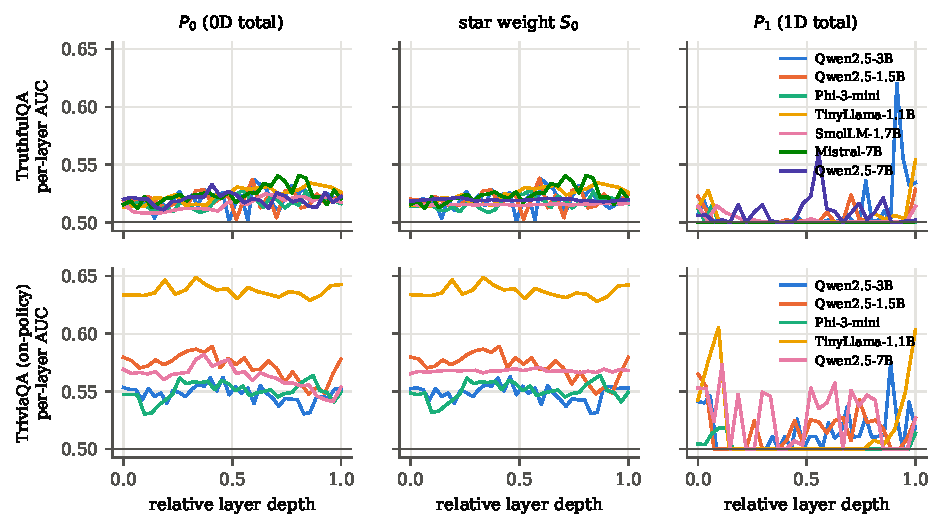
\includegraphics[width=\linewidth]{fig_sink_layer_auc.pdf}\caption{\textbf{Single-feature AUC by layer.} Curves need per-example layer features, which we retain for 15 of the 16 settings (not TrQA Mis7B). Mistral-7B is shown in its \texttt{[INST]} format only.}\label{fig:layerauc}\end{figure}

\paragraph{Worked example.} Figure~\ref{fig:example} shows TruthfulQA question 67 with its incorrect answer (``Yes, vampires are real'') under TinyLlama-1.1B ($N{=}29$). In layer 5 the model sends 0.85 of its attention to token 0 on average, $\defect_0=0.000$, and accordingly $P_0=4.225$ equals the star weight $\stw_0=4.225$ and there are 0 $H_1$ bars. In layer 21 sink attention drops to 0.53 and $\defect_0=0.281$; now $P_0=12.287$ falls below $\stw_0=13.043$ (within the bound $(N{-}2)\defect_0=7.59$), and 10 $H_1$ bars appear, the longest of length 0.172$\,\le\defect_0$. The theorem bounds loops but does not force them: in layers 2 and 11--18 of the same example $\defect_0$ lies between $0.11$ and $0.52$, yet $H_1$ is empty.
\begin{figure}[H]\centering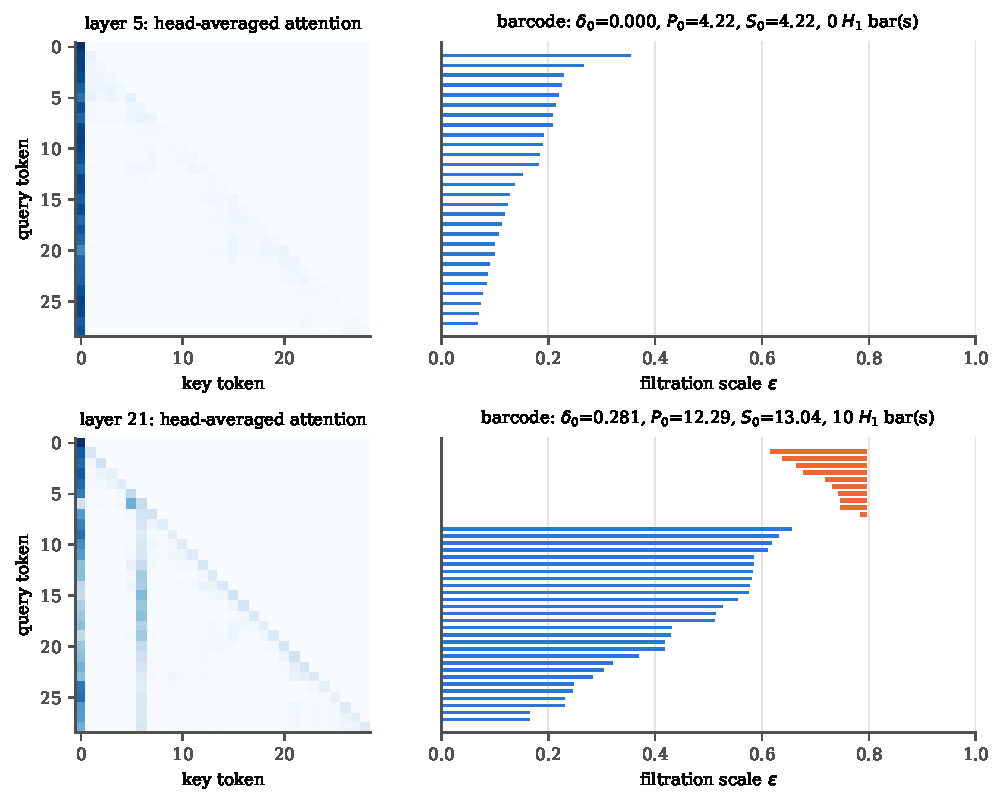
\includegraphics[width=\linewidth]{fig_sink_example.pdf}\caption{\textbf{A coned and a non-coned layer of the same example} (TinyLlama-1.1B, TruthfulQA). Left: head-averaged attention; the bright first column is the sink. Right: $0$D bars (blue) and $1$D bars (orange) of the Vietoris--Rips filtration of $D=1-\max(A,A^\top)$.}\label{fig:example}\end{figure}
